\documentclass[a4paper, landscape]{article}
\usepackage{prerex}
\usepackage{multicol}
%\usepackage{showframe}
\usetikzlibrary{calc}
\usepackage[utf8]{inputenc} % codificacao de caracteres
\usepackage{geometry}
\usepackage{tikz}
\tikzset{
    %Define standard arrow tip
    >=stealth,
    %Define style for boxes
    box/.style={
           rectangle,
           draw=black,
           text width=7em,
           minimum height=5em,
           text centered,
           inner sep=1mm]},
    % Define arrow style
    pil/.style={
           ->,
           thick,
           shorten <=3pt,
           shorten >=3pt,},
}
\usetikzlibrary{positioning,shapes,shadows,arrows}
\tikzstyle{basico}=[box, fill=yellow]
\tikzstyle{desc}=[box, fill=orange]
\tikzstyle{profissional}=[box, fill=green]
\tikzstyle{eletiva}=[box, fill=orange!50!white, dashed]
\newcounter{cred}
\setcounter{cred}{0}
\newcounter{thoras}
\setcounter{thoras}{0}
\newcommand{\disciplina}[8] {
  \addtocounter{cred}{#7}; \addtocounter{thoras}{#6};
  \node at ($ (#2*2.8-3,15-#3*2.3) $) (Item)  [#1] (#8) 
        {
            \textbf{#4}\\
            \textbf{#5}\\
            \textbf{#6} \hfill #7
        };}
\newcommand{\prereq}[2] {
  \draw [->, thick](#1.east)--(#2.west);}
%nó acima
\newcommand{\prereqAcima}[2] {
   \draw [->, thick]
    ($(#1.east) + (0,2mm) $) %comece 2mm abaixo de east 
    -| ($ (#2.west)+(-3mm,-2mm)$) %quebre 90º até chegar a 3mm ao lado e 2 abaixo de west 
    -- ($(#2.west)-(0,2mm)$); %termine 2 mm abaixo de west
    }
\newcommand{\prereqAbaixo}[2] {
   \draw [->, thick]
    ($(#1.east) + (0,-2mm) $) %comece 2mm abaixo de east  
    -| ($ (#2.west) -(3mm,-2mm)$) %quebre 90º até chegar a 3mm ao lado e 2 abaixo de west
    -- ($(#2.west) + (0,2mm)$); termine 2 mm acima de west
    }
\newcommand{\prereqNivelAbaixo}[2] {
   \draw [->, thick]
    ($(#1.east) + (0,-2mm) $) -| ($(#1.east) + (3mm,-15mm) $) -| ($ (#2.west) -(2mm,-2mm)$) -- ($(#2.west) + (0,2mm)    $);}
\newcommand{\prereqA}[2] {
   \draw [->, thick]
    ($(#1.east) + (0,2mm) $) -| ($(#1.east) + (2mm,15mm) $) -| ($ (#2.west) -(2mm,0)$) -- ($(#2.west)    $);}
\newcommand{\prereqB}[2] {
  \draw [->, thick]
    ($(#1.east) + (0,-1mm) $)  -| ($ (#2.west) -(1mm,-4mm)$) -- ($(#2.west) + (0,4mm)    $);}
\geometry{margin=1cm,bottom=1.5cm} 
  
\begin{document}
\noindent
{\Large \textbf{Curso: Engenharia}}\\
{\Large \textbf{Habilitação: Sistemas e Computação}}

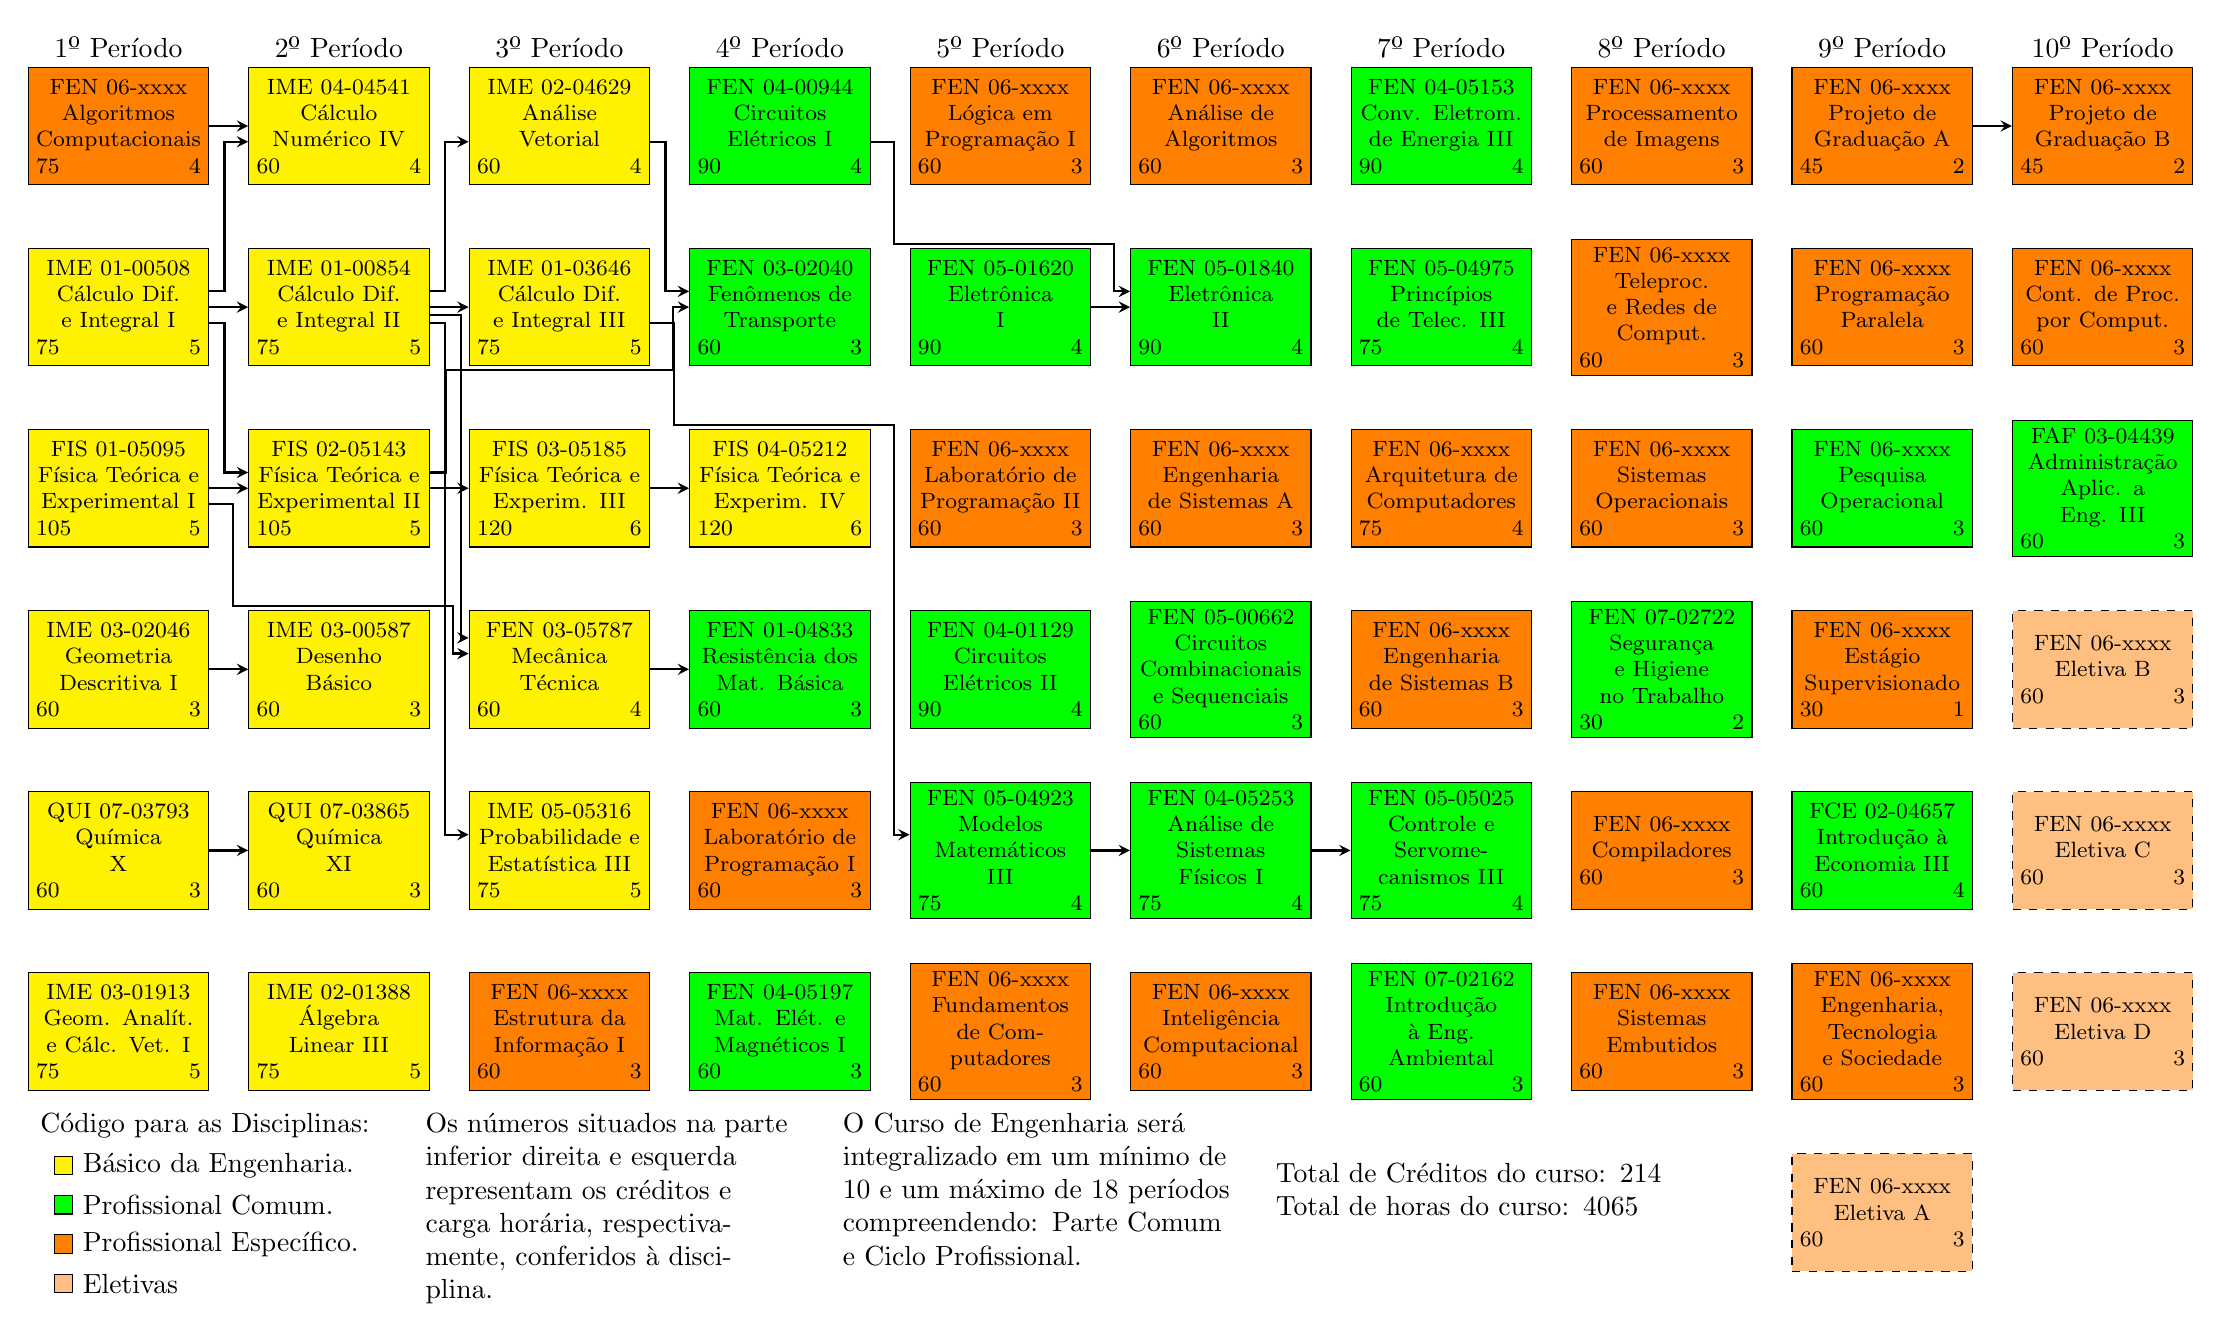
\begin{tikzpicture}
\foreach \x in {1,...,10} {\node at (\x*2.8-3,13.7) {\xº Período};}

\footnotesize 
\fontfamily{anttlc}
%parâmetros de cada disciplina, pode ser posto numa única linha
%\disciplina
%{basico || profissional || desc || eletiva}
%{Período} de 1 a 10
%{Linha no fluxograma} de 1 a 6.
%{Código da disciplina}
%{Nome da Disciplina}
%{Carga Horária}
%{Número de Créditos}
%{nome abreviado para referência}

%Básico
\disciplina{basico}{2}{6}{IME 02-01388}	{Álgebra\\ Linear III}{75}{5}{AlgLin}
\disciplina{basico}{2}{6}{IME 02-01388}	{Álgebra\\ Linear III}{75}{5}{AlgLin}
\disciplina{basico}{3}{1}{IME 02-04629}	{Análise\\ Vetorial}{60}{4}{AnaVet}
\disciplina{basico}{1}{2}{IME 01-00508}	{Cálculo Dif. e Integral I}{75}{5}{CalcI}
\disciplina{basico}{2}{2}{IME 01-00854}	{Cálculo Dif. e Integral II}{75}{5}{CalcII}
\disciplina{basico}{3}{2}{IME 01-03646}	{Cálculo Dif. e Integral III}{75}{5}{CalcIII}
\disciplina{basico}{2}{1}{IME 04-04541}	{Cálculo Numérico IV}{60}{4}{CalcNum}
\disciplina{basico}{2}{4}{IME 03-00587}	{Desenho\\ Básico}{60}{3}{DesBas}
\disciplina{basico}{1}{3}{FIS 01-05095}	{Física Teórica e\\Experimental I}{105}{5}{FisI}
\disciplina{basico}{2}{3}{FIS 02-05143}	{Física Teórica e\\Experimental II}{105}{5}{FisII}
\disciplina{basico}{3}{3}{FIS 03-05185}	{Física Teórica e\\Experim. III}{120}{6}{FisIII}
\disciplina{basico}{4}{3}{FIS 04-05212}	{Física Teórica e\\Experim. IV}{120}{6}{FisIV}
\disciplina{basico}{1}{4}{IME 03-02046}	{Geometria Descritiva I}{60}{3}{GD}
\disciplina{basico}{1}{6}{IME 03-01913}	{Geom. Analít.\\ e Cálc. Vet. I}{75}{5}{GeoAna}
\disciplina{basico}{3}{4}{FEN 03-05787}	{Mecânica\\ Técnica}{60}{4}{MecTec}
\disciplina{basico}{3}{5}{IME 05-05316}	{Probabilidade e\\ Estatística III}{75}{5}{ProbEst}
\disciplina{basico}{1}{5}{QUI 07-03793}	{Química\\ X}{60}{3}{QuiX}
\disciplina{basico}{2}{5}{QUI 07-03865}	{Química\\ XI}{60}{3}{QuiXI}

%disciplinas profissional
\disciplina{profissional}{10}{3}{FAF 03-04439}	{Administração Aplic. a Eng. III}{60}{3}{Adm}
\disciplina{profissional}{6}{5}	{FEN 04-05253}	{Análise de Sistemas Físicos I}{75}{4}{AnaFis}
\disciplina{profissional}{4}{1}	{FEN 04-00944}	{Circuitos Elétricos I}{90}{4}{CEI}
\disciplina{profissional}{5}{4}	{FEN 04-01129}	{Circuitos Elétricos II}{90}{4}{CEII}
\disciplina{profissional}{7}{5}	{FEN 05-05025}	{Controle e Servomecanismos III}{75}{4}{ServoMec}
\disciplina{profissional}{7}{1}	{FEN 04-05153}	{Conv. Eletrom. de Energia III}{90}{4}{ConvEle}
\disciplina{profissional}{5}{2}	{FEN 05-01620}	{Eletrônica\\ I}{90}{4}{EletI}
\disciplina{profissional}{6}{2}	{FEN 05-01840}	{Eletrônica\\ II}{90}{4}{EletII}
\disciplina{profissional}{4}{2}	{FEN 03-02040}	{Fenômenos de Transporte}{60}{3}{FenTran}
\disciplina{profissional}{9}{5}	{FCE 02-04657}	{Introdução à Economia III}{60}{4}{IntEco}
\disciplina{profissional}{7}{6}	{FEN 07-02162}	{Introdução à Eng. Ambiental}{60}{3}{IntAmb}
\disciplina{profissional}{4}{6}	{FEN 04-05197}	{Mat. Elét. e Magnéticos I}{60}{3}{MatEle}
\disciplina{profissional}{5}{5} {FEN 05-04923}	{Modelos Matemáticos III}{75}{4}{ModMat}
\disciplina{profissional}{7}{2}	{FEN 05-04975}	{Princípios de Telec. III}{75}{4}{PrincTelec}
\disciplina{profissional}{4}{4}	{FEN 01-04833}	{Resistência dos Mat. Básica}{60}{3}{ResMat}
\disciplina{profissional}{8}{4}	{FEN 07-02722}	{Segurança e Higiene no Trabalho}{30}{2}{SegHig}

%Disciplinas Desc
\disciplina{desc}{1}{1} {FEN 06-xxxx}	{Algoritmos\\Computacionais}{75}{4}{AlgComp}
\disciplina{desc}{6}{1} {FEN 06-xxxx}	{Análise de Algoritmos}{60}{3}{AnAlg}
\disciplina{desc}{7}{3} {FEN 06-xxxx}	{Arquitetura de Computadores}{75}{4}{ArqComp}
\disciplina{profissional}{6}{4}	{FEN 05-00662}	{Circuitos Combinacionais e Sequenciais}{60}{3}{CirComb}
\disciplina{desc}{8}{5} {FEN 06-xxxx}	{Compiladores}{60}{3}{Comp}
\disciplina{desc}{10}{2}{FEN 06-xxxx}	{Cont. de Proc. por Comput.}{60}{3}{Control}
\disciplina{desc}{9}{6} {FEN 06-xxxx}	{Engenharia, Tecnologia e Sociedade}{60}{3}{ETS}
\disciplina{desc}{6}{3} {FEN 06-xxxx}	{Engenharia de Sistemas A}{60}{3}{EnsSistA}
\disciplina{desc}{7}{4} {FEN 06-xxxx}	{Engenharia de Sistemas B}{60}{3}{EngSistB}
\disciplina{desc}{9}{4} {FEN 06-xxxx}	{Estágio Supervisionado}{30}{1}{EstSup}
\disciplina{desc}{3}{6} {FEN 06-xxxx}	{Estrutura da Informação I}{60}{3}{EstrInf}
\disciplina{desc}{5}{6} {FEN 06-xxxx}	{Fundamentos de Computadores}{60}{3}{FundComp}
\disciplina{desc}{6}{6} {FEN 06-xxxx}	{Inteligência Computacional}{60}{3}{IC}
\disciplina{desc}{4}{5} {FEN 06-xxxx}	{Laboratório de Programação I}{60}{3}{LabProgI}
\disciplina{desc}{5}{3} {FEN 06-xxxx}	{Laboratório de Programação II}{60}{3}{LabProgII}
\disciplina{desc}{5}{1} {FEN 06-xxxx}	{Lógica em Programação I}{60}{3}{LogProg}
\disciplina{profissional}{9}{3} {FEN 06-xxxx}	{Pesquisa Operacional}{60}{3}{PO}
\disciplina{desc}{8}{1} {FEN 06-xxxx}	{Processamento de Imagens}{60}{3}{ProcImag}
\disciplina{desc}{9}{2} {FEN 06-xxxx}	{Programação Paralela}{60}{3}{ProParal}
\disciplina{desc}{9}{1} {FEN 06-xxxx}	{Projeto de Graduação A}{45}{2}{ProjA}
\disciplina{desc}{10}{1}{FEN 06-xxxx}	{Projeto de Graduação B}{45}{2}{ProjB}
\disciplina{desc}{8}{6} {FEN 06-xxxx}	{Sistemas Embutidos}{60}{3}{SistEmb}
\disciplina{desc}{8}{3} {FEN 06-xxxx}	{Sistemas Operacionais}{60}{3}{SO}
\disciplina{desc}{8}{2} {FEN 06-xxxx}	{Teleproc. e Redes de Comput.}{60}{3}{TeleRed}

%eletivas
\disciplina{eletiva}{9}{7} {FEN 06-xxxx}	{Eletiva A}{60}{3}{EA}
\disciplina{eletiva}{10}{4}{FEN 06-xxxx}	{Eletiva B}{60}{3}{EB}
\disciplina{eletiva}{10}{5}{FEN 06-xxxx}	{Eletiva C}{60}{3}{EC}
\disciplina{eletiva}{10}{6}{FEN 06-xxxx}	{Eletiva D}{60}{3}{ED}

\prereq{CalcI}{CalcII}
\prereq{CalcII}{CalcIII}
\prereqAcima{CalcI}{CalcNum}
\prereq{FisI}{FisII}
\prereq{FisII}{FisIII}
\prereq{FisIII}{FisIV}
\prereqAbaixo{CalcII}{ProbEst}
\prereq{GD}{DesBas}
\prereq{EletI}{EletII}
\prereq{ProjA}{ProjB}
\prereq{QuiX}{QuiXI}
\prereq{AlgComp}{CalcNum}
\prereqAbaixo{CalcI}{FisII}
\prereqNivelAbaixo{FisI}{MecTec}
\prereqAcima{CalcII}{AnaVet}

\prereqA{FisII}{FenTran}
\prereqB{CalcII}{MecTec}

\prereq{MecTec}{ResMat}
\prereq{ModMat}{AnaFis}
\prereq{AnaFis}{ServoMec}

\prereqNivelAbaixo{CalcIII}{ModMat}
\prereqNivelAbaixo{CEI}{EletII}
\prereqAbaixo{AnaVet}{FenTran}


%\filldraw[color=yellow, draw=black] rectangle (0.3,0.3) at (\textwidth/10,15-7*2.3);
\normalsize 
\node at (0.9cm,0) (legenda){Código para as Disciplinas:};
\node at (-0.9cm,-0.5) [fill=yellow, draw=black, label=right:Básico da Engenharia.] (basico) {};
\node [below  of=basico,node distance=5mm,fill=green, draw=black, label=right:Profissional Comum.] (prof) {};
\node [below of=prof,node distance=5mm,fill=orange, draw=black, label=right:Profissional Específico.] (especifico){};
\node [below of=especifico,node distance=5mm,fill=orange!50!white, draw=gray, draw=black, label=right:Eletivas] {};

\node at (6cm,-1.05) [ text width=4.6cm] {Os números situados na parte inferior direita e esquerda representam os créditos e carga horária, respectivamente, conferidos à disciplina.};

%tirando duas eletiva
\addtocounter{thoras}{-120} 
\addtocounter{cred}{-6}


\node at (11.5cm,-0.8) [ text width=5cm]
{O Curso de Engenharia será integralizado em um mínimo de 10 e um máximo de 18 períodos compreendendo: Parte Comum e Ciclo Profissional.};

\node at (17,-0.8) [ text width=5cm] {Total de Créditos do curso: \the\value{cred}\\
Total de horas do curso: \the\value{thoras}};
\end{tikzpicture}

\raggedright
\begin{multicols}{3}


\columnbreak






\columnbreak


\end{multicols}

\end{document}
